\chapter{Design of a Query Plan-Aware Partitioning Advisor}
\chaptermark{Query Plan-Aware Partitioning Advisor}
\label{Methods}

\section{Deep Neural Network Architecture \& Hyper Parameters}
A typical Deep-Q-Learning architecture consists of an \textit{input layer}, multiple \textit{hidden layers} and one \textit{q-value} output layer. A common, but successful architecture style uses densely connected layers to form the Q-network, as established in \cite{DBLP:journals/corr/MnihKSGAWR13}. For our project, we use the architecture described in Table~\ref{tab:neural-network-architecture}. Additionally, we also incorporate a \textit{Lambda} layer to resize the input layer to the size of the \textit{state-action} pair. 

% Please add the following required packages to your document preamble:
% \usepackage[table,xcdraw]{xcolor}
% If you use beamer only pass "xcolor=table" option, i.e. \documentclass[xcolor=table]{beamer}
\begin{table}[ht]
  \centering
    \begin{tabular}{|l|l|l|l|}
\hline
\rowcolor[HTML]{DAE8FC} 
\textbf{Layer (type)}  & \textbf{Output Shape} & \textbf{Param \#} & \textbf{Activation} \\ \hline
input\_1 (Input Layer) & {[}(None, 177){]}     & 0                 & None                \\ \hline
lambda\_1 (Lambda)     & (None, 157)           & 0                 & None                \\ \hline
dense\_1 (Dense)       & (None, 128)           & 20224             & 'relu'              \\ \hline
dense\_2 (Dense)       & (None, 64)            & 8256              & 'relu'              \\ \hline
dense\_3 (Dense)       & (None, 1)             & 65                & 'linear'            \\ \hline
\end{tabular}
    \caption{Deep-Q Neural Network Architecture}
    \label{tab:neural-network-architecture}
\end{table}

In terms of hyper-parameters, Table~\ref{tab:hyp-param} surmises our choices. The hyper-parameters were tuned empirically for the best results.

% Please add the following required packages to your document preamble:
% \usepackage[table,xcdraw]{xcolor}
% If you use beamer only pass "xcolor=table" option, i.e. \documentclass[xcolor=table]{beamer}
\begin{table}[ht]
\centering
    \begin{tabular}{|l|l|}
    \hline
    \rowcolor[HTML]{DAE8FC} 
    \textbf{Hyper-Parameter} & \textbf{Value} \\ \hline
    Optimiser                & Adam           \\ \hline
    $\epsilon$-decay         & 0.997          \\ \hline
    $\gamma$ (discount-rate) & 0.99           \\ \hline
    $\alpha$ (learning-rate) & $5 \cdot 10^{-4}$         \\ \hline
    $\tau$ (target network update) & $10^{-3}$ \\ \hline
    Experience Replay Buffer Size & 10000 \\ \hline
    Batch Size for Experience Relay & 32 \\ \hline
    Episodes & 600/1000 \\ \hline
    \end{tabular}
    \caption{Hyper-Parameters for training.}
    \label{tab:hyp-param}
\end{table}

\section{Revisiting the Problem-Formulation}
A partitioning problem can be formally described as follows: Given a set of tables \textit{T} and queries \textit{Q}, for every table $T_i \in T$ with attributes $a_{i1},a_{i2},...,a_{in}$ we have to decide whether to replicate or to partition the table. For our approach, we only consider horizontal partitioning schemes using \textit{hash-partitioning}, which horizontally splits a table into a fixed number of shards (which is equal to the number of nodes in the database cluster). Thus, when two tables use the same partitioning attribute, we assume that they are co-partitioned on that attribute and equi-joins on that attribute do not involve any data-shuffling. For replication, we make a simplifying assumption: if a table is replicated, it is replicated to all nodes in the cluster. 
To summarise, in order to solve the partitioning problem, for each table, we thus have to decide whether that table is partitioned or replicated \cite{Hilprecht:2019:TLP:3329859.3329876}. If it is partitioned, we additionally need to decide which attribute $a_i$ (or set of attributes) is being used for horizontal partitioning.
In their original work, \citeauthor{Hilprecht:2019:TLP:3329859.3329876}'s main intuition to model partitioning as a DRL problem was to model the database and the query workload as state and possible changes to the partitioning scheme as actions. In the following section, we first go through \citeauthor{Hilprecht:2019:TLP:3329859.3329876}'s version, and our proposed changes to the state-action pair.

\section{State}
A deep reinforcement learning neural network takes the state-action pair as input to the model to derive a Q-value for all possible actions, i.e. which partitioning or replicating actions to take. Therefore, it is quite fundamental to design the state in a manner that provides the model inference capabilities based on the state of the database cluster. In game playing learning scenarios such as teaching the agent how to play Atari \cite{DBLP:journals/corr/MnihKSGAWR13}, the state is encoded as the pixels of the game for any given frame. For such tasks, encoding the state is quite a straightforward approach, i.e. the pixels represent the state, $s_t$ at timestep $t$. With regard to the database partitioning task, we follow the general approach of \citeauthor{Hilprecht:2019:TLP:3329859.3329876}, and design the state vector with the following considerations:


\subsection{Replication and Partition state}
For every table $T_i$, we have to encode whether it is currently partitioned or replicated. If it is partitioned, we additionally have to encode which attribute(s) are used for partitioning. Hence, for each table, we can encode its state as a binary vector using one-hot encoding:
\begin{equation}
    s(T_i) = (r_i, a_{i1},a_{i2},...,a_{in})
\end{equation}
In order to vectorise the state of the entire table, we concatenate each vector to produce, $s(T) = s(T_1)^\frown s(T_2)^\frown ...^\frown s(T_n)$, where $n$ is the total number of tables.

\subsection{Workload Frequency}
The workload frequency for each query in the query workload $Q$ is also modelled as part of the state. For the same database schema, different workload frequencies would result in different optimal partitioning strategies that should be selected. For the purposes of this work, we assume that every possible query $q_i$ in a workload of queries $Q$ is known in advance. Given this scenario, the query workload can be represented as a vector where an entry encodes the frequency $f_i$ for a query $q_i$:
\begin{equation}
\label{eq:workload-frequency}
    s(Q) = (f_1,...,f_m)
\end{equation}
where $m$ is the total number of queries in the workload mix. The frequencies are normalised and hence, we obtain a vector where the entries are in the interval $[0,1]$. 

\subsection{Co-Partitioning Edges}
We capture co-partitioning of two tables using the concept of edges, which come about in order to limit the search space and prevent sub-optimal partitioning schemes. As a result, we extend the state representation pushing the agent to explore only partitioning schemes where the tables are co-partitioned. To this end, every foreign key-primary key relationship between the attributes $a_{ir}$ and $a_{js}$ of the corresponding tables $T_i$ and $T_j$ includes an edge $(T_i,a_{ir},T_j,a_{js})$ which can either be active or inactive. If active, our approach guarantees that both relations are co-partitioned by that attribute if we perform a join between the two relations on that attribute, i.e. $T_i$ is hash-partitioned by $a_{ir}$ and $T_j$ is hash-partitioned by $a_{js}$. For example in Figure~\ref{fig:state-rep}, the edge $e_1$ is active and thus \texttt{lineorder} and \texttt{customer} table must be partitioned by the attributes \texttt{lo\_custkey} and \texttt{c\_custkey} respectively.



\begin{figure}[h]
  \centering
  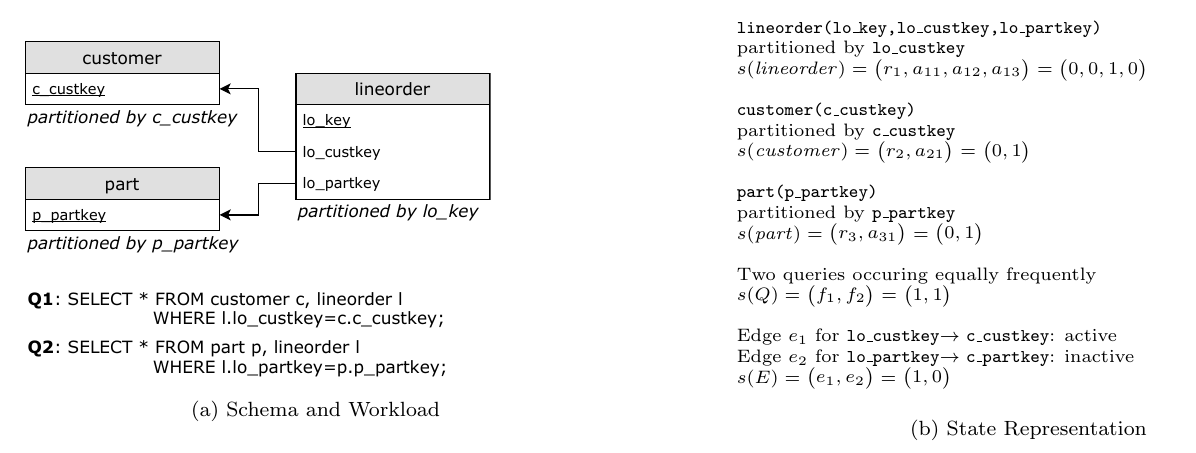
\includegraphics[width=\linewidth]{figures/simplified-ssb-schema-workload.png}
  \caption{Simplified SSB Schema and Workload}
  \label{fig:state-rep}

\end{figure}

\subsection{Modelling the Query and Query Optimiser as State}
\citeauthor{Hilprecht:2019:TLP:3329859.3329876} used the strategies discussed above in order to model the state for the DRL agent. However, there are a few limitations in the modelling above:
\begin{itemize}
    \item \textbf{Query Features} - Despite modelling the query workload frequencies as state, the rich features from the individual queries are not included in the state. 
    \item \textbf{Query Optimiser} - At no point is the cost information from the query optimiser used to model the state either. 
\end{itemize}

\subsection{Distributed Database - System X}
\label{sec:system-x}
In order to fully understand the following methodology, we must first discuss the choice of the distributed database system whose query optimiser we wish to use in our partitioning advisor. In our work, we are using a commercial distributed database which supports SQL, \textbf{in-memory} rowstore tables and disk-backed columnstore tables. For licensing reasons, we will refer to this system in the following as \textbf{System-X}. System-X was built specifically for horizontal-scale out architectures and its primary feature - in-memory rowstore design circumvents many of the issues that arise with disk-based databases. All of its functionalities can be used through a MySQL wire protocol-compatible interface. The rowstore requires that all the data can fit in main memory. By completely avoiding disk IO, System-X makes use of a variety of techniques to speed up the execution, with minimal principal latencies. System-X supports two kinds of nodes in a cluster, i) \textbf{leaf} nodes store data and ii) \textbf{aggregator} nodes coordinate DML. One of the aggregator nodes is "master" and coordinates DDL. One of our major contribution is towards integrating System-X's query-optimiser as part of the DRL agent's state. Like most query-optimisers, System-X's query-optimiser generates plans for every query. But more importantly, System-X's query optimiser also provides insights about the distributed nature of the query alongside other key operations.

Before we move on to the next section, we have to make an important distinction as to how we define the term \textit{optimiser cost}. While System-X's query optimiser does use cost-based optimisation to find minimum cost-estimated query plans, it does not expose cost-estimates. However, we use \textbf{cardinality estimates} (or row estimates) provided by System-X's query optimiser as a proxy to estimate compute costs and network costs. Henceforth, optimiser costs only refer to the row estimates we receive from the query optimiser.

\subsection{Obtaining Query Optimiser Costs}
\label{sec:obt-query-opt-costs}
The cost information captures the cost of processing the query. However, a query usually has many possible physical plans and each plan has a different query cost. So it is not realistic to directly parse the query statement to extract the query cost. Instead, we generate query features using the query plan generated by the query optimiser, which has a cost estimate for each operation. System-X's query-optimiser generates the best plans for each query based on statistical analysis of the rows in each relation. The query plans also expose \textit{statistical row estimates} for key operations for each query. For example, consider the following scenario:

\begin{listing}[ht]
\inputminted[frame=lines,
            breaklines=true,
            framesep=2mm,
            fontsize=\footnotesize]
            {sql}
            {listings/query-optimiser-code.sql}
\caption{Example code to generate query-plan}
\label{listing:query-optimiser-code}
\end{listing}

Listing~\ref{listing:query-optimiser-code} generates the following query plan.

\begin{figure}[h]
  \centering
  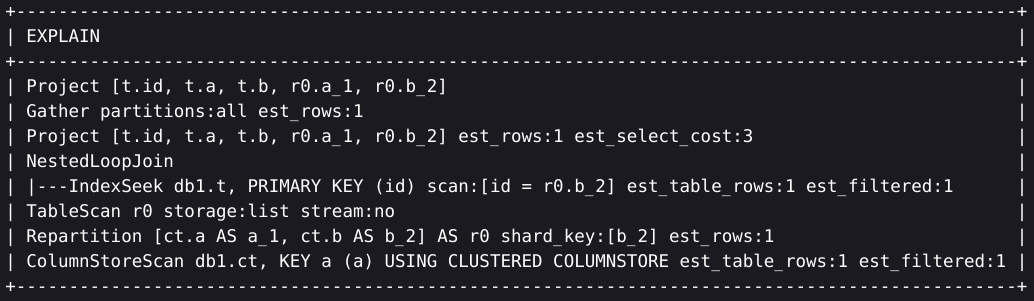
\includegraphics[width=\linewidth]{figures/explain-example.png}
  \caption{Example query plan generated for Listing~\ref{listing:query-optimiser-code}}
  \label{fig:explain-example}
\end{figure}

In total, System-X supports up to \textbf{17} operations. However, since our problem domain is the partitioning problem, not all operations are valuable to us. As such, we focus on the following operations:
\begin{itemize}
        \item Joins
        \begin{enumerate}
            \item \texttt{HashJoin} - performs a hash join: System-X builds a hash table from the results of the inner side of the join and probes into it while scanning the outer part of the join
            \item \texttt{MergeJoin} - performs a merge join: System-X scans both inner and outer sides of the join at the same time and merges matching rows
            \item \texttt{NestedLoopJoin} - performs a NestedLoop join: for every row on the outer side of the join System-X seeks or scans into the inner table to find all the matching rows
        \end{enumerate}
        \item Distributed Data Movement
        \begin{enumerate}
            \item \texttt{Gather} - collects all the results from the leaf nodes to the aggregator node. 
            \item \texttt{GatherMerge} - collects ordered streams of rows from the leaves and merges them to output an ordered stream
            \item \texttt{Repartition} - redistributes a dataset to hash-partition it on a particular key
            \item \texttt{Broadcast} - broadcasts a dataset to every node in a cluster
        \end{enumerate}
\end{itemize}
From this point, we will only be considering the \textit{estimated row counts} of the aforementioned operations. However, an astute observer might notice from Figure~\ref{fig:explain-example} that none of the join operations have any estimated row counts. A simple approach we took in order to calculate the cost of each join was by aggregating the total row count of each table access operation performed for each join. Consider the following query and its corresponding query plan, Figure~\ref{fig:tpc-ch-query-02-plan}.

\begin{listing}[ht]
\inputminted[frame=lines,
            breaklines=true,
            framesep=2mm,
            fontsize=\footnotesize]
            {sql}
            {listings/tpc_ch_02.sql}
\caption{TPC-CH Query 02}
\label{listing:tpc-ch-query-02}
\end{listing}

System-X supports 5 different kinds of table access methods, among which two are \texttt{ColumnStoreScan} and \texttt{OrderedColumnStoreScan}, both of which are only applicable for column-store tables. Since our approach only utilises row-store tables, we do not worry about the column-store based table access methods. As such, we only consider the following three table access methods:

\begin{itemize}
    \item \texttt{TableScan} - scans every row in a table using an index
    \item \texttt{IndexSeek} - navigates to a particular row using an index
    \item \texttt{IndexRangeScan} - scans a range of rows using an index
\end{itemize}

\begin{figure}[ht]
  \centering
  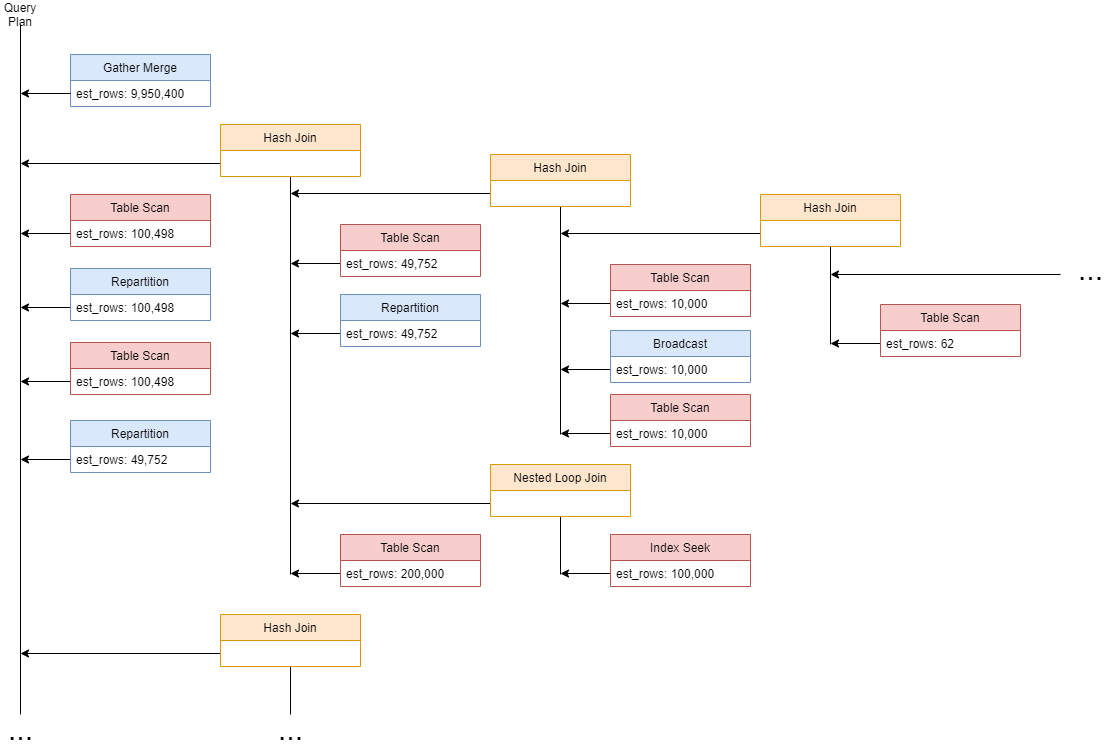
\includegraphics[width=\linewidth]{figures/query_02_plan_01.png}
  \caption{A section of the query plan for Listing~\ref{listing:tpc-ch-query-02}}
  \label{fig:tpc-ch-query-02-plan}
\end{figure}

In Figure~\ref{fig:tpc-ch-query-02-plan}, table access operations are illustrated in red, join operations in yellow and all other operations in blue. The rest of the diagrams will remain thematically consistent with this approach. Once we calculate the join costs, the query plan could be illustrated as in Figure~\ref{fig:join-cost-calculation}.

\begin{figure}[ht]
  \centering
  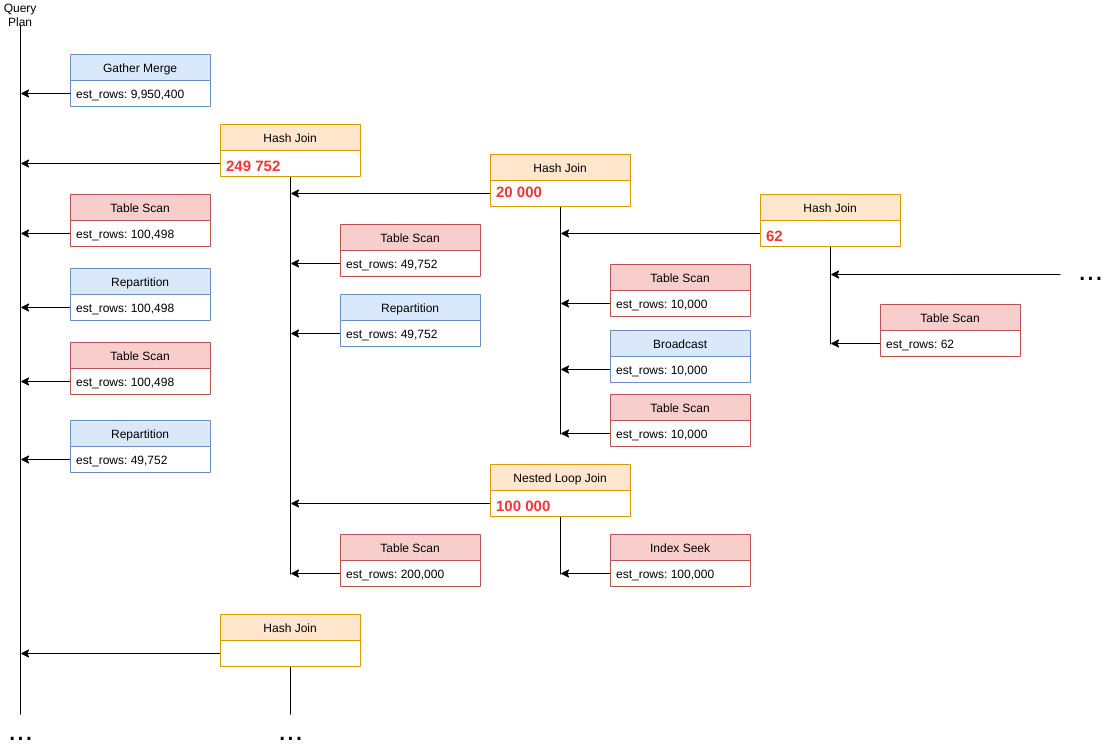
\includegraphics[width=\linewidth]{figures/query_02_plan_02.png}
  \caption{Join cost calculation for TPC-CH Query 02}
  \label{fig:join-cost-calculation}
\end{figure}


\subsection{Intuition for Query Optimiser and Query Featurisation}
However, before we explain how the query optimiser and query features are integrated into the model, let's try to understand the intuition behind why integrating the state of the query workload and the optimiser could be beneficial. Consider the following query, which is the 5th query from the TPC-CH benchmark.

\begin{listing}[ht]
\inputminted[frame=lines,
            breaklines=true,
            framesep=2mm,
            fontsize=\footnotesize]
            {sql}
            {listings/tpc_ch_05.sql}
\caption{TPC-CH Query 05}
\label{listing:tpc-ch-query-05}
\end{listing}

This query can be used to highlight how different partitioning schemes can give rise to different optimal query plans. For example, this query requires multiple equi-joins between several relations on several attributes, such as:
    \begin{itemize}
        \item \texttt{c\_id = o\_c\_id}
        \item \texttt{ol\_o\_id = o\_id}
        \item \texttt{ol\_i\_id = s\_i\_id}
    \end{itemize}
From the perspective of a database administrator, if we were to try to optimise this query for performance, we would like for the two biggest relations, in this case \texttt{orders} and \texttt{orderline} to be co-partitioned. Given that we would like to optimise this query, we could come up with the following partitioning scheme:
    \begin{itemize}
        \item orderline \texttt{SHARD KEY (ol\_o\_id, ol\_w\_id, ol\_d\_id)}
        \item orders \texttt{SHARD KEY (o\_id, o\_w\_id, o\_d\_id)}
        \item enable local reference joins between the two largest relations and reduce re-partitioning costs.
        \item consider a partitioning scheme where all tables are replicated except for \texttt{orderline} and \texttt{orders} which are co-partitioned.
    \end{itemize}

The complete plan generated by query-05 from Listing~\ref{listing:tpc-ch-query-05} for the optimised partitioning scheme can be found in Appendix~\ref{appendix:1}. System-X's query optimiser is capable enough to understand that this query does not require any \texttt{Repartitioning} or \texttt{Broadcast} operations since all relations are either replicated and relations which have a join between them are co-partitioned. This query plan is visually represented in Figure~\ref{fig:tpc-ch-query-05-plan}. For brevity, the table access methods are not displayed. 


Now consider an un-optimal partitioning scheme, where \texttt{orders} and \texttt{orderline} are not co-partitioned. For example:
    \begin{itemize}
        \item orderline \texttt{SHARD KEY (ol\_i\_id, ol\_d\_id)}
        \item orders \texttt{SHARD KEY (o\_w\_id, o\_d\_id)}
        \item This would mean that the two relations aren't co-partitioned, which would involve some repartitioning and shuffling costs generated by the query optimiser.
    \end{itemize}
Surely enough, System-X's query optimiser recognises that and produces the plan generated in Appendix~\ref{appendix:2} which has been visualised in Figure~\ref{fig:tpc-ch-query-05-plan-unopt}. The un-optimised query plan contains repartitioning costs owing to the two relations not being co-partitioned. Modelling this key information as part of the environment aims to provide the agent with more information about the current state of the query optimiser, similar to how a database administrator would optimise the query. Following this intuition, we discuss how we featurise our queries and feed it into the neural network model.


\begin{figure}
     \centering
     \begin{subfigure}[b]{0.45\textwidth}
          \centering
          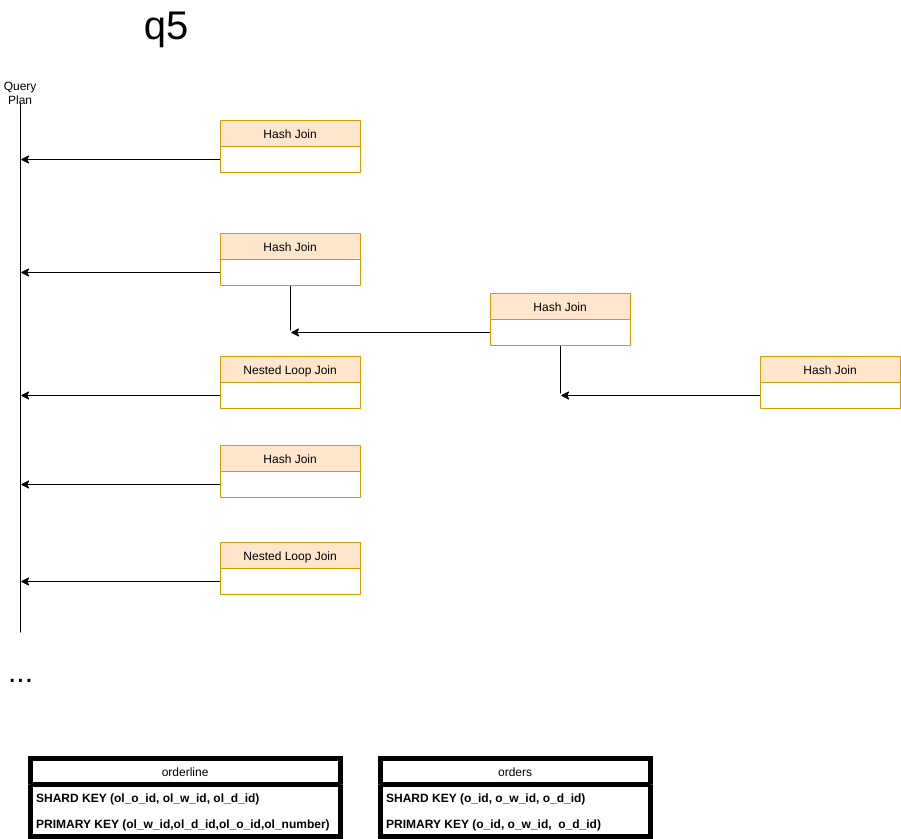
\includegraphics[height=10cm]{figures/query_05_plan_01_opt.png}
          \caption{Optimised}
          \label{fig:tpc-ch-query-05-plan}
     \end{subfigure}
     \hfill
     \begin{subfigure}[b]{0.45\textwidth}
          \centering
          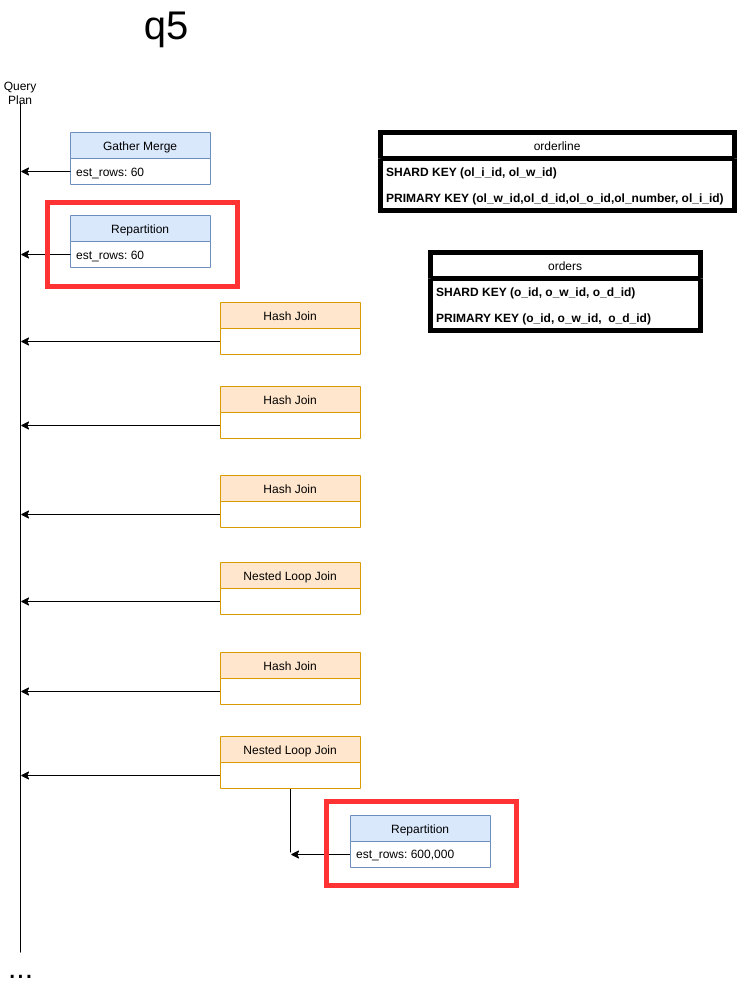
\includegraphics[height=10cm]{figures/query_05_plan_01_unopt.png}
          \caption{Un-optimised}
          \label{fig:tpc-ch-query-05-plan-unopt}
     \end{subfigure}
     \caption{Optimal and un-optimised query plans for TPC-CH Query 05.}
\end{figure}

\subsection{Query Featurisation}
In this section, we focus on how the query, and subsequently how the query workload is featurised and fed into the deep reinforcement learning model. As in Figure~\ref{fig:join-cost-calculation}, an operation may appear in different nodes of the tree plan, and the cost of the same operation should be summed up as the corresponding cost value in the query cost vector. For example, in Figure~\ref{fig:join-cost-calculation}, the value of the hash join equals to the sum of the costs in all the Hash Join nodes. After gaining the query cost, we normalise the cost by subtracting mean and dividing the standard deviation. This step is necessary to enforce the \textit{generalisability} of our model to any query workload and \textit{reduce} the number of weights required to train the model.

In summary, for cost information, we maintain a $|P|$ dimensional vector, where $P$ is the set of operations in database, and $|P|$ is the number of operations, where $P = 7$ in our approach, similar to \cite{DBLP:journals/pvldb/LiZLG19}.

\begin{equation}
    v = (\sum o_1, \sum o_2, ... \sum o_7)
\end{equation}
\begin{equation}
    v_{norm} = \frac{v - \mu(v)}{\sigma(v)}
\end{equation}
    

\subsubsection{Vector for Multiple Queries}
Given a query workload has multiple queries, $q_1, q_2, ... , q_m$, suppose the cost vectors generated for those are $v_1, v_2, ..., v_m$ respectively. In order to feed each individual vector into the DRL agent, we need to combine the vectors together. We take a simple approach by summing up the costs and produce a vector for the query optimiser and query workload, $O$ as follows:
\begin{equation}
    s(O) = \sum_{1}^{m} v_i
    \label{eq:first-s(O)}
\end{equation}
where $|s(O)| = P$. In this aspect of the query featurisation, one might wonder why we would combine the queries into a single vector. Combining the vector serves two purposes: i) \textit{generalisation} of the query workload and ii) reducing the \textit{search space} required for training the DRL model.  

Consider an alternative plan, where the individual query cost vectors are not combined together, but rather appended together. This alternative scheme would produce a vector as follows:
\begin{equation}
    s(O) = (\ v_1^\frown v_2^\frown ...^\frown v_m\ )
    \label{eq:second-s(O)}
\end{equation}
In this scheme, $|s(O)| = m*P$. Now consider the Deep-Q Learning architecture which was used to train the model, as illustrated in Table~\ref{tab:neural-network-architecture}. Given that our first hidden layer has 128 neurons, using the second featurisation style~\ref{eq:second-s(O)} would involve training $(m-1)*P*128$ weights over the first one~\ref{eq:first-s(O)}. In addition to removing the \textit{generalisability} of the model to adapt to a query workload of any size, it would also involve additional overhead in the number of weights, which are required for training as $m$ grows larger, i.e. if the query workload becomes larger, thus increasing the search space. As such, we opt for a more statistical driven approach by summing up the cost vectors.

In summary, we augment \citeauthor{Hilprecht:2019:TLP:3329859.3329876}'s model by modelling the state as:
\begin{equation}
    s = s(T)^\frown s(Q)^\frown s(O)
\end{equation}

\section{Action}
An action represents some way of the agent interacting with the environment to change the state of the environment. As such, the number of possible actions depend on the state of the environment. For the same reasons, a small state space is essential to apply Q-learning because for making the decision which action to execute in a state, we have to compute the Q-values for all possible actions. Hence, the agent can only take actions which change only one aspect of the partitioning encoded in the state at a time.
Consider a simple example, where we have a singe table $T_i$. The agent can either replicate the table or partition it by one of its attributes, $a_{ir}$. These actions are only considered if the table is currently in a physical state that does not conflict with the target state, e.g. replicate the table $T_i$ is only a valid action if the table is not already replicated. To that end, the actions are restricted to only those which do not conflict with the current set of active edges. For example, replicating table $T_i$ is not a valid action if the edge $(T_i,a_{ir},T_j,a_{js})$ is active because otherwise the guarantee that $T_i$ is partitioned by $a_{ir}$ and $T_j$ is partitioned by $a_{js}$ would not hold anymore.
The agent is also capable of taking a second class of actions. These actions make the use of edges as short-cuts to change the partitioning scheme. In summary, activating an edge co-partitions two tables while the de-activation of edges is also possible. The activation of edges must also be conflict-free, and so the agent checks that in the set of edges, there are no two edges which require a table $T_i$ to be partitioned by different attributes $a_{ir}$ and $a_{ir'}$. For example, in Figure~\ref{fig:state-rep}, edge $e_2$ cannot be activated as $e_1$ is already active.
Furthermore, as an additional contribution to the previous work done by \citeauthor{Hilprecht:2019:TLP:3329859.3329876}, we also introduce compound-key co-partitioning edges. This allows the agent to consider compound-key sharding strategies. However, this does increase the search-space for the DRL agent. Given that the complexity of training using Deep Reinforcement Learning is $O(|s|^3)$ \cite{DBLP:conf/aaai/KoenigS93}, the tight bound still remains the same, but the size of the state grows larger.
\section{Reward}
The overall goal is to find a partitioning scheme that minimises the runtime of the set of queries $Q$ modeled as part of the input state. Since this objective has to be minimised by the DRL agent, it can be used as a reward. We use the actual runtimes $c_r(P,q_i)$ of the queries $q_i$ given a partitioning $P$ or alternatively use a cost model $c_m(P,q_i)$ approximating the true runtime. In fact, the actual costs are used for the online training phase and the cost model costs are used for the offline training phase. For simplicity, in the following, we just assume one cost function $c(P,q_i)$ that reflects the runtime of the query $q_i$ over partitioning $P$.
The DRL agent is designed to maximise the reward, but we want to minimise the costs. As such, we use negative costs in the reward definition. However, instead of simply designing the reward as $\sum^m_{j=1}f_j*c(P,q_j)$, we additionally normalise the reward with respect to a reference partitioning scheme, $P_0$, for example, a partitioning scheme where all the tables are replicated in the database cluster.
\begin{equation}
    r = - \frac{\sum^m_{j=1}f_j*c(P,q_j)}{\sum^m_{j=1}f_j*c(P_0,q_j)}
\end{equation}

\section{Offline Phase}
As mentioned previously, the DRL agent uses the offline cost model for training this phase. Since we introduce the query optimiser only in the online training phase, the offline phase needs to incorporate a \textit{dummy state} for the query optimiser throughout the offline training phase. This is achieved through simply feeding a vector $v_{dummy} = (0, 0, 0, 0, 0, 0, 0) $ as the query optimiser state to the offline model. This is an empirical approach as the offline and online model input layers need to be compatible with each other. Owing to feeding $0$s to the offline-model, the offline model does not learn the weights $\theta$ for the query optimiser. These weights are later refined in the online phase where the query optimiser costs are actually integrated. Besides these optimisations, the offline phase remains identical to the work performed in \cite{DBLP:conf/sigmod/HilprechtBR20}. 

% algorithm 
\begin{algorithm}
    \begin{algorithmic}[1]
        \caption{Offline Training} \label{algorithm:offline-training}
        \State Randomly initialise Q-network $Q_\theta$
        \State Randomly initialise target network $Q_{\theta'}$
        \For{e in 0, 1, ..., $e_{max}$} \Comment{Episodes}
            \State Reset state to $s_0$
            \For{t in 0, 1, ..., $t_{max}$} \Comment{Steps in Episode}
                \State Calculate $s_{t+1}$
                \State Choose $a_t = \argmax_a Q_\theta(s_{t+1},a)$ with probability $1-\epsilon$, otherwise random action
                \State Execute action $a_t$, i.e. simulate what the next state $s_{t+1}$ and partitioning $P_{t+1}$ would be
                \State Compute reward with cost model $c_m$:
                \State $\frac{\sum^m_{j=1} f_jc_m(P_{t+1},q_j)}{\sum^m_{j=1} f_jc_m(P_0,q_j)}$
                \State Store transition $(s_t, a_t, r_t, s_{t+1})$ in B
                \State Sample minibatch $(s_i, a_i, r_i, s_{i+1})$ from B
                \State Train Q-Network with SGD and loss
            \EndFor
            \State $\sum^b_{i=1}(r_i + \gamma \argmax_{a \in A} Q_{\theta'} (s_{i+1},a) - Q_\theta (s_i, a_i))^2$
            \State Decrease $\epsilon$
            \State Update weights of target model: $\theta' = (1-\tau)\theta' + \tau \theta$
        \EndFor
    \end{algorithmic}
\end{algorithm}

\section{Online Phase}
\label{sec:online-training}
In contrast to offline training, the idea of online training is to actually deploy the partitionings $P_i$ corresponding to the visited states $s_i$ on a database cluster and measure the true runtimes $c_r(P_i,q_i)$ to compute the reward. A naive approach would be to run the online training from the start and finish at the maximum number of episodes. In practice, this is way to oexpensive to be used. Imagine that there are 1000 episodes and each having $t_{max}=100$ steps which is one of the hyperparameter settings we used in our experiments. Assuming we have a schema and a query workload which takes on average 20 minutes to run, and each repartitioning episode takes another 20 minutes. If we simply executed every action the agent proposes, i.e. we repartition the tables and measure the workload times on the cluster, we would end up with a runtime of $(20 \textit{mins} + 20 \textit{mins})*1000*100 \approx 7.6 \textit{years}$. As such, the online training is only performed to refine the model produced by the offline training phase. Hence, one approach is to use the pre-trained offline-agent and further train it with real runtimes. This has no effect if we use the same degree of exploration, i.e., if we choose random actions with the same probabilities $1-\epsilon$. In DRL training, the $\epsilon$ value is decayed by a factor called the $\epsilon-\textit{decay}$ after each episode. Therefore, we start the online training with an epsilon value which is reached after 600 episodes in the first episode. This drastically reduces the training runtime of the online phase. Even with an optimisation such as this, \citeauthor{Hilprecht:2019:TLP:3329859.3329876} implement a few more optimisation techniques for the online training phase which are briefly discussed as follows:
% \subsubsection{Sampling} Only talk about this if time to evaluate workload frequencies
\subsubsection{Runtime Caching}
Runtime caching can be justified by the fact that if the DRL agent visits two states $s_i$ and $s_j$ during training and they have the same corresponding partitioning $P$ then the rewards $r_i$ and $r_j$ must be identical. This naive approach can be further refined by keeping a state of the tables associated with each query. That is to say, if the partitionings $s_i$ and $s_j$ only differ for a certain set of tables $\{T_{i1}, T_{i2},...,T_{in}\}$ we only have to run queries that contain at least one of those tables. For every query, we can maintain a table containing the different state combinations $s(T_{i1}),s(T_{i2}),...,s(T_{in})$ and the runtime of the query on the dataset. In summary, when visiting a new query, we examine the state of every table $s(T_i)$, i.e. whether it is replicated or partitioned by an attribute(s), and only run the queries $q_i$ for which we do not have a runtime entry for the state combination of the relevant tables.
\subsubsection{Query Feature Caching}
Whenever a new state $s_i$ is visited, we use a similar technique to Runtime Caching to store Query Features in a Query Feature Cache. This assumes that System-X's query optimiser will produce the same query plan for a given set of state combinations $s(T_{i1}),s(T_{i2}),...,s(T_{in})$. This allows us to reduce the number of times the database cluster needs to be queried for the state features during the online training phase, and is also necessary for the model inference which will be described shortly.

\subsubsection{Lazy Repartitioning}
Lazy Repartitioning results as an implementation of Query Runtime Caching. It is an offshoot of Query Runtime Caching, because the intuition is that if the rewards for the state $s_i$ being visited has already been visited, then we do not need to perform the action which was suggested by the DRL agent. As such, the rewards can be calculated again from the Query Runtime Cache, and proceed to the next timestep for queries where this table is involved have to be measured. The approach of lazy repartitioning is to keep track of the partitioning deployed on the database $P_{actual}$ and the partitioning $P_t$ of the state $s_t$ the agent is currently at. Every time the agent chooses an action and we reach a new state we first check which queries $\{q_{j1}, . . . , q_{jn}\}$ have to be executed on the database. Especially in later phases of training this will be significantly fewer queries than the full set $Q$ since many runtimes will be in the Query Runtime Cache.

\subsubsection{Timeouts}
Timeouts are a necessary result of queries that take too long to run for a given partitioning scheme, which are obviously not optimal. Hence, we can safely abort the query execution and move on with the training. The reward for an aborted query is defined to be:
\begin{equation}
    r = - \frac{\sum^m_{j=1}f_js_j(P,q_j)}{C}
\end{equation}
where C is an empirical value chosen through experimentation for the given workload. If a query $q_i$ takes longer than $C$, the query is aborted. In practice, however, this is further refined by keeping an replica of a small dataset along with the large dataset that the agent partitions simultaneously. If the query runtime is greater than $C$ on the smaller dataset, it is skipped.

\subsubsection{Penalising Non-Runnable Queries}
\label{sec:penalise-query}
Here, we introduce an optimisation solely for System-X. With System-X, some queries fail to run on certain partitioning schemes owing to feature-limitations in System-X. A similar principle to Timeouts is used in this case, where non-runnable queries are penalised with a higher cost, so that the agent learns to avoid the partitioning state that led to non-runnable queries.

\subsubsection{Overall Procedure}
Combining these optimisations, we observe training algorithm 2 for online training. Note that in line 10, when $s_{t+1}$ is calculated, the query featuriser is used to determine the new state of the query optimiser as well after $P_{t+1}$ is simulated on the database.

% algorithm 
\begin{algorithm}
    \begin{algorithmic}[1]
        \caption{Online Training} \label{algorithm:online-training}
        \State Sample from full dataset and deploy tables with initial partitioning on cluster
        \State Initialise $P_{actual}$
        \State Randomly initialise Q-network $Q_\theta$
        \State Randomly initialise target network $Q_{\theta'}$
        \State Initialize Query Runtime Cache C = \{\}
        \For{e in 0, 1, ..., $e_{max}$} \Comment{Episodes}
            \State Reset state to $s_0$
            \For{t in 0, 1, ..., $t_{max}$} \Comment{Steps in Episode}
                \State Choose $a_t = \argmax_a Q_\theta(s_{t+1},a)$ with probability $1-\epsilon$, otherwise random action
                \State Execute action $a_t$, i.e. simulate what the next state $s_{t+1}$ and partitioning $P_{t+1}$ would be
                \State Determine set of queries $Q_t$ which have to be run on $P_{t+1}$ because of missing values in C
                \State \textit{// Lazy Repartitioning}
                \State Determine set of tables $T_{Qt}$ contained in $Q_t$
                \For{ $T_i$ in $T_{Qt}$}
                    \If{ $T_i$ is different in $P_{actual}$ and $P_{t+1}$}
                        \State Repartition $T_i$ according to $P_{t+1}$
                        \State Update $P_{actual}$
                    \EndIf 
                    \State \textit{// Fill Query Runtime Cache}
                \EndFor
                \For{ $q_i$ in $Q_t$}
                    \State Measure $t = c_{sample}(P_{t+1},q_i)$ by running $q_i$
                    \State Determine the states of relevant tables for $q_i$:
                    \State $(s(T_{i1}),...,s(T_{in}),t)$ in C
                \EndFor
                \State \textit{// Exploit Query Runtime Cache}
                \State Lookup costs $c_{sample}(P_{t+1},q_i)$ in C
                \State Compute reward $r_t = \frac{\sum^m_{j=1} f_js_jc_{sample}(P_{t+1},q_j)}{\sum^m_{j=1} f_js_jc_{sample}(P_0,q_j)}$
                \State Store transition $(s_t, a_t, r_t, s_{t+1})$ in B
                \State Sample minibatch $(s_i, a_i, r_i, s_{i+1})$ from B
                \State Train Q-Network with SGD and loss
            \EndFor
            \State $\sum^b_{i=1}(r_i + \gamma \argmax_{a \in A} Q_{\theta'} (s_{i+1},a) - Q_\theta (s_i, a_i))^2$
            \State Decrease $\epsilon$
            \State Update weights of target model: $\theta' = (1-\tau)\theta' + \tau \theta$
        \EndFor
    \end{algorithmic}
\end{algorithm}

\subsubsection{Model Inference}
Having trained the DRL agents, we now describe how they can be used to obtain partitionings. In order to obtain the inference, we start with a reference initial state $s_0$, where all the tables are replicated. We iteratively choose the action that maximises the Q-function, i.e. $a_t = \argmax_aQ_\theta(s_{t+1},a)$. This is similar to setting $\epsilon = 0$ or full exploitation and no exploration at all. We execute $t_max$ actions and obtain a sequence of states, actions and rewards. Owing to caching both the query runtimes and the query features, we don't need to query the cluster at all and perform the model inference independently of the cluster. Since the DRL agent is trained to maximise the reward, this trajectory will contain states $s_t$ which lead to high rewards, i.e. the queries of the workload have short runtimes on the corresponding partitionings $P_t$. \citeauthor{Hilprecht:2019:TLP:3329859.3329876} observe that the DRL agent tends to oscillate around the optimal partitioning $P^*$ in this sequence. Moreover, due to caching the query features for every visited state, we can follow the same procedure as using cached rewards.
